The history about this term begins near the year 2008 \cite{DefineGamefication}. 
It was coined to summarise the use of game elements on non-game contexts.
In the year 2010 the term reached the critical mass to appear on Google
Trends\cite{LiCap1.3}.

The idea of this concept initially was use on the 80s to make an upgrade to a 
game called MUD \emph{Multy User Dungeons}. The person behind this was Richard Bartle
who begin to analise the people who played this games and found 4 stereotypes of
players,\ref{fig:Players}.

With this types of players he developed a new MUD to satisfy each type of player.
After the sucess of the idea of focus certein aspects of the game to engage the players
the non-game industry began to use game elements to engage people over their products. 

\begin{figure}[!htb]
  \centering
  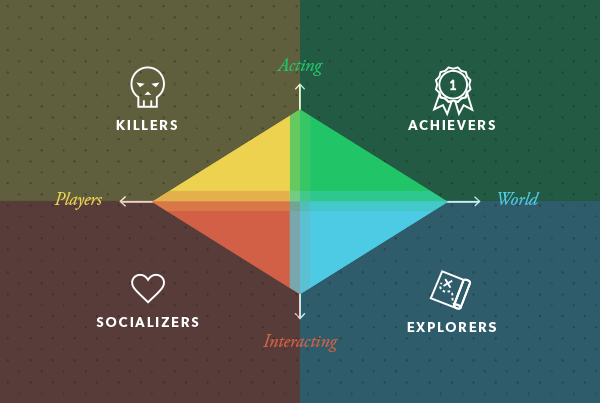
\includegraphics[width=0.5\textwidth]{images/TypeOfPlayersBartle.png}
  \caption[Caption for LOF]{Real caption\footnotemark}
  \label{fig:Players}
\end{figure}

\footnotetext{Source: \url{http://www.example.com/theimage.png}}
 	


Nowadays Gamification has become a really useful tool to engage people. With this in mind
the industry and people using it needs a description to unite all diferent concepts
about Gamification so everyone can understand it and begin to work with a unique conception.
Gamificaton is \emph{the use of game design elements in non-game related contexts}. 
Within the definition are four concepts that are very important to understand.

\begin{itemize}

\item Game:

\item Element:

\item Design:

\item Non-Game Context:

\end{itemize}

Gamification can be use on multiple context where the attention of the user is needed. Some of this context are education, sales and marketing.

\begin{itemize}

\item Education: In this context the use of gamification can be seen in different ideas to engage the
the students and keep them interested. Some of this concepts can be use in schools and universities
where the students are 

\item Sales and marketing:

\end{itemize}

